%!TEX program = xelatex

\documentclass[czech]{beamer}
\usetheme{Dresden}
\usecolortheme{beaver}

%\usepackage[utf8]{inputenc}
%\usepackage[T1]{fontenc}

%\usepackage{tgadventor}

\usepackage{fontspec}
\setsansfont{Segoe UI Semilight}

\usepackage{pgfplots}

\defbeamertemplate*{headline}{miniframes theme no section}
{%
	\begin{beamercolorbox}[colsep=1.5pt]{upper separation line head}
	\end{beamercolorbox}
	\begin{beamercolorbox}{section in head/foot}
 		\vskip2pt\insertnavigation{\paperwidth}\vskip2pt
	\end{beamercolorbox}
	\begin{beamercolorbox}[colsep=1.5pt]{lower separation line head}
	\end{beamercolorbox}
}

\setbeamertemplate{section in toc}[sections numbered]

\begin{document}	
	\title{GPU-based speedup of EACirc project}
	\author[Jiří Novotný]{\begin{tabular}{r l}Author: &Jiří Novotný\\Supervisor: &RNDr. Petr Švenda, Ph.D.\end{tabular}}
	\institute{Faculty of Informatics\\Masaryk University}
	\date{Spring 2015}

	\frame{\titlepage}
	
	\begin{frame}
		\frametitle{Outline}
		\tableofcontents
	\end{frame}
	
	\section{Introduction \& Objective}
	\begin{frame}
		\frametitle{What is EACirc?}
		\centering
		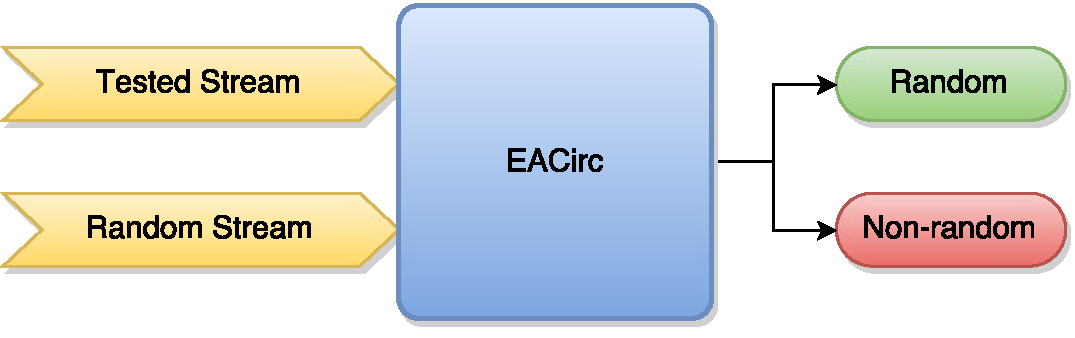
\includegraphics[width=.8\textheight]{eacirc}
		
		\bigskip
		Distinguishes input streams from one another.
	\end{frame}
	
	\begin{frame}
		\frametitle{How EACirc works?}
		\centering
		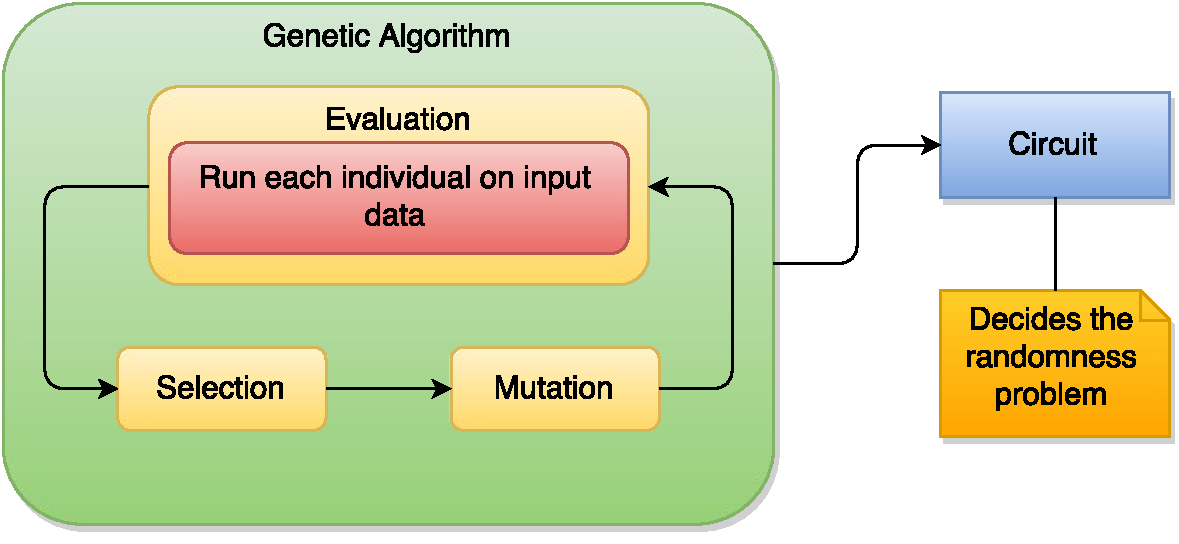
\includegraphics[width=.7\textwidth]{ga}
		
		\medskip
		\small{Speeding-up the evaluation could move the EACirc capabilities further.}
	\end{frame}
	
	\section{Solution}
	\begin{frame}
		\frametitle{CUDA}
		 CUDA is a platform enabling general purpose computing on GPU.
		 
		 \bigskip
		\begin{columns}[c]
			\begin{column}{.45\textwidth}
				\centering
				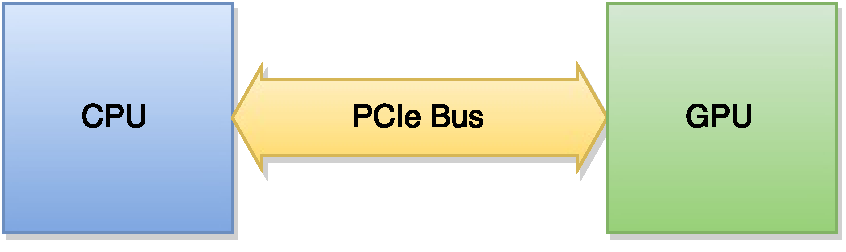
\includegraphics[width=\textwidth]{hpc}
				
				\medskip
				\small{Different device \& architecture}
			\end{column}
			\hfill\vline\hfill
			\begin{column}{.45\textwidth}
				\centering
				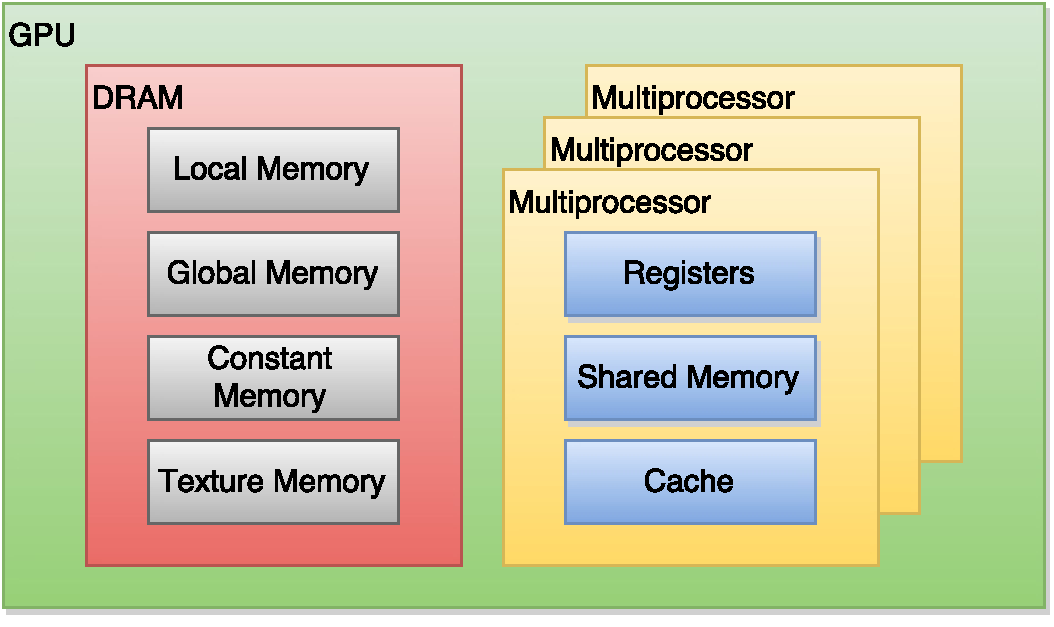
\includegraphics[width=\textwidth]{memory}
				
				\medskip
				\small{Complex memory design}
			\end{column}
		\end{columns}
	\end{frame}
	
	\section{My contribution}
	\begin{frame}
		\frametitle{GPU circuit}
		\begin{columns}[T]
			\begin{column}{.6\textwidth}
				\begin{itemize}
					\item natural data parallelism
					\item different implementation than the original circuit due to the CUDA memory restrictions
				\end{itemize}
			\end{column}
			\hfill\vline\hfill
			\begin{column}{.4\textwidth}
				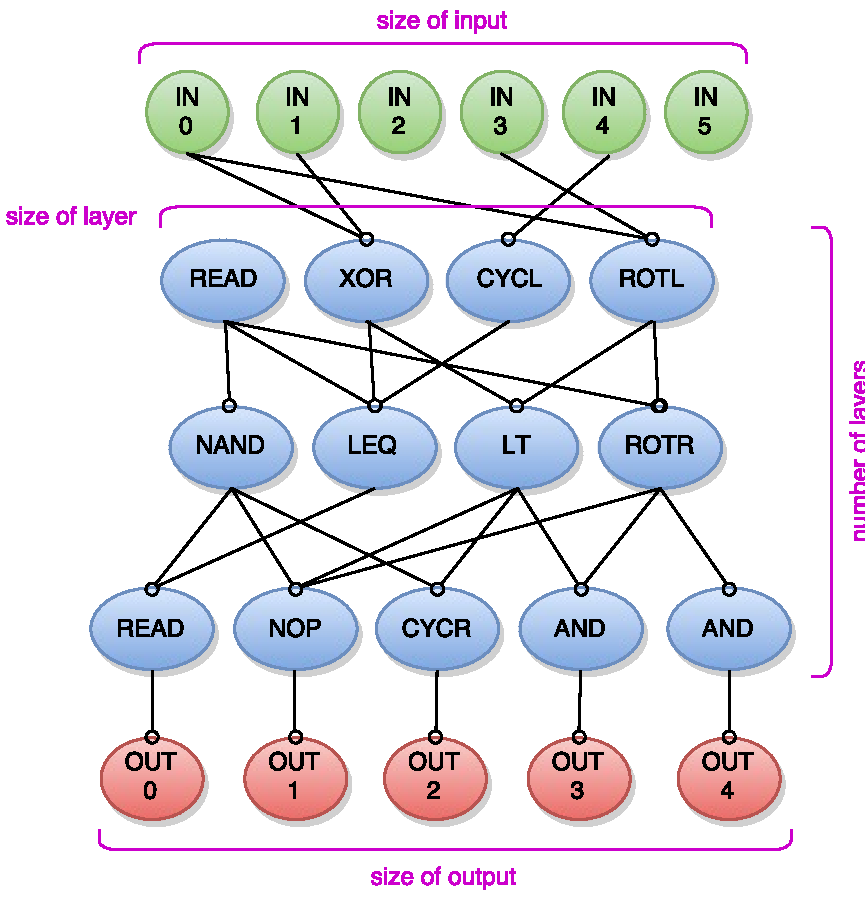
\includegraphics[width=\textwidth]{circuit}
			\end{column}
		\end{columns}
	\end{frame}
		
	\begin{frame}
		\frametitle{Benchmarks}
		\centering
		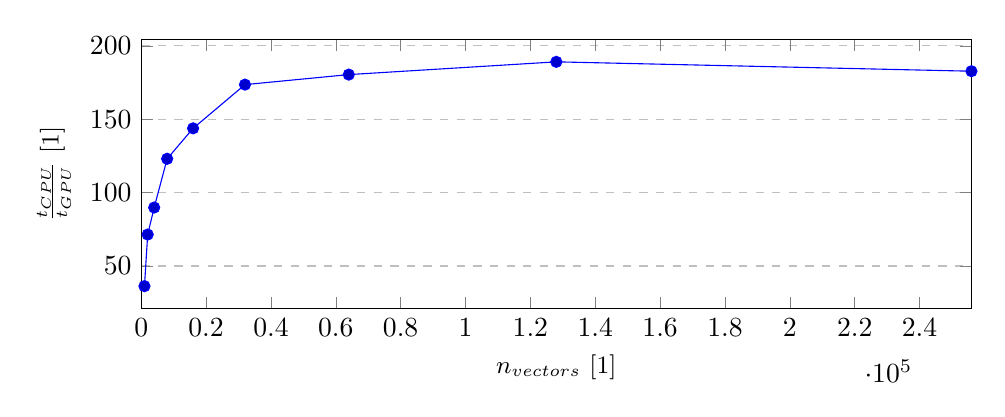
\begin{tikzpicture}
			\begin{axis}[
			width=\textwidth,height=5cm,
			xlabel={\small{$n_{vectors}$ [$1$]}},
			ylabel={\small{$\frac{t_{CPU}}{t_{GPU}}$ [$1$]}},
			log ticks with fixed point,
			xmin=0, xmax=256000,
			ymajorgrids=true,
			grid style=dashed,
			legend pos=north west,
			]
			\addplot coordinates {
				(1000, 36.29)(2000, 71.45)(4000, 89.84)(8000, 123.04)(16000, 143.78)(32000, 173.57)(64000, 180.39)(128000, 189.08)(256000, 182.7)
			};
			\end{axis}
		\end{tikzpicture}
	\end{frame}
	
	\begin{frame}
		\frametitle{The new build-system}
		\begin{itemize}
			\item CUDA needs different building process
			\item previously for each platform a separate makefile
			\item hard to maintain
		\end{itemize}
		\bigskip
		\begin{itemize}
			\item solved by CMake integration
			\item separation of EACirc modules into static libraries
		\end{itemize}
	\end{frame}
	
	\section{Summary}
	\begin{frame}
		\frametitle{Summary}
		\begin{columns}[c]
			\begin{column}{.5\textwidth}
				The GPU circuit
				\begin{itemize}
					\item designed to utilize the GPU
					\item implemented
					\item integration tested
					\item benchmarked on GeForce GTX~460
					\item 160x speed-up
					\item expected to be integrated into production
				\end{itemize}
			\end{column}
			\hfill\vline\hfill
			\begin{column}{.5\textwidth}
				The new build-system
				\begin{itemize}
					\item easy to maintain
					\item conditional building of modules \& features
					\item refactored filesystem structure
					\item integrated into production
				\end{itemize}
			\end{column}
		\end{columns}
	\end{frame}
\end{document}